\chapter{Background}
\label{chap:Background}

The research problem outlined in Section~\ref{sec:Research_Problem_and_Scope} cannot be addressed with a single technology. Our solution was to develop a method that integrates OWL+SWRL, Prolog and DTMC and PCTL\@. OWL was chosen because it is an established knowledge representation formalism, and the ontology specification language recommended by the W3C~\cite{Horrocks_2011}. OWL limitations motivate several contending extensions including SWRL, CARIN, $\mathcal{AL}$-log, DL-safe rules, $\mathcal{DL}$+log, and many others~\cite{Motik_2006}. Hybrid knowledge representation systems that integrate OWL+SWRL and Prolog have also been proposed~\cite{Sensoy_2011,Matzner_2007,Papadakis_2011,Samuel_2008,Lukacsy_2009a,Almendros_Jimenez_2011,Elenius_2012}. We chose to address OWL limitations with SWRL and Prolog; the former is an OWL extension approved by the W3C, while the latter is one of the most prominent logic-based knowledge representation languages.

Probabilistic model checking is supported by various software tools including ProbVerus and FMur$\varphi$, which analyze DTMC models; ETMCC and MRMC (the successor of ETMCC), which analyze DTMC and CTMC models; and LiQuor and Rapture, which analyze MDP models~\cite{Baier_2008}. But PRISM is, in our opinion, preferable because it supports both model types, thereby extending the potential of our method and prototype. PRISM also supports PCTL, a formalism that can express a large class of properties in an elegant manner.

The remainder of this chapter is structured as follows. Section~\ref{sec:OWL_SWRL_and_Prolog} investigates the formal logics underpinning OWL+SWRL and Prolog to determine the advantages and limitations of each formalism, and their compatibility with each other. Section~\ref{sec:Probabilistic_Model_Checking} presents model checking, probabilistic model checking, and the DTMC and PCTL formalisms. Section~\ref{sec:UAV_Missions} provides an overview of the UAV domain and complex UAV missions with a focus on UAV \emph{performance specifications}, \emph{mission aspects} and \emph{mission scenarios}. This chapter is summarized in Section~\ref{sec:Background_Summary}.

\section{OWL+SWRL and Prolog}
\label{sec:OWL_SWRL_and_Prolog}

\emph{Description logics} (DLs) are a family of knowledge representation languages based on \emph{first-order logic} (FOL) that can be used to construct logically valid knowledge bases. DLs describe a domain in terms of \emph{concepts} or \emph{classes} (specified as axioms in a TBox), \emph{individuals} (specified as assertions in an ABox) and \emph{properties} or \emph{roles}~\cite{Horrocks_2011}. DL concepts and individuals are roughly comparable to classes and objects, respectively, in object-oriented programming, while roles are comparable to UML associations.

An interpretation $\mathcal{I}$ is a model of a TBox $\mathcal{T}$ and an ABox $\mathcal{A}$ \emph{iff} $\mathcal{I}$ satisfies all axioms and assertions in $\mathcal{T}$ and $\mathcal{A}$, respectively. More formally, an interpretation $\mathcal{I} = (\Delta^\mathcal{I}, \cdot^\mathcal{I})$ comprises a non-empty set $\Delta^\mathcal{I}$ (the domain of $\mathcal{I}$) and a function $\cdot^\mathcal{I}$ that maps:

\begin{itemize}

\item every concept $A_i$ to a subset $A_i^\mathcal{I}$ of $\Delta^\mathcal{I}$ ($A_i^\mathcal{I} \subseteq \Delta^\mathcal{I}$);

\item every role $R_i$ to a binary relation $R_i^\mathcal{I}$ over $\Delta^\mathcal{I}$ ($R_i^\mathcal{I} \subseteq \Delta^\mathcal{I} \times \Delta^\mathcal{I}$);

\item and every individual $a_i$ to an element $a_i^\mathcal{I}$ of $\Delta^\mathcal{I}$ ($a_i^\mathcal{I} \in \Delta^\mathcal{I}$).

\end{itemize}

DLs support inferences that deduce the logical implications of ontological axioms with respect to concept \emph{satisfiability}, \emph{subsumption}, \emph{equivalence} and \emph{disjointness}~\cite{Baader_2005}. TBox-supported inference services can be formalized as follows:

\begin{itemize}

\item a concept $C$ is satisfiable with respect to a TBox $\mathcal{T}$ \emph{iff} there exists some model $\mathcal{I}$ of $\mathcal{T}$ such that $C^\mathcal{I} \not= \emptyset$;

\item $C$ is subsumed by a concept $B$ with respect to $\mathcal{T}$ \emph{iff} $C^\mathcal{I} \subseteq B^\mathcal{I}$ for all $\mathcal{I}$ of $\mathcal{T}$;

\item $C$ is equivalent to $B$ with respect to $\mathcal{T}$ \emph{iff} $C^\mathcal{I} = B^\mathcal{I}$ for all $\mathcal{I}$ of $\mathcal{T}$;

\item $C$ is disjoint from $B$ with respect to $\mathcal{T}$ \emph{iff} $C^\mathcal{I} \cap B^\mathcal{I} = \emptyset$ for all $\mathcal{I}$ of $\mathcal{T}$.

\end{itemize}

OWL is an ontology specification language based on the modern description logic $\mathcal{SHOIN(\mathbf{D})}$~\cite{Horrocks_2011}. The OWL language structures, and thereby supports the automated processing of, formalized knowledge. But OWL is constrained by the expressive and reasoning limitations inherent in $\mathcal{SHOIN(\mathbf{D})}$. For example, OWL can be used to model object relations that form tree-like patterns, but not the triangular relationship that exists between a child, the child's father, and the father's brother~\cite{Motik_2006}; nor the self-referential relationship that references an individual to itself~\cite{Krotzsch_2011}. SWRL addresses some of these limitations by extending OWL with Horn-like rules~\cite{Horrocks_2004}. But OWL+SWRL cannot reason effectively with negation~\cite{Motik_2006,McGrath_2008}. Problems that are intractable in OWL+SWRL can be addressed with the programming language Prolog~\cite{Motik_2006,Volz_2003}.

Prolog is based on a FOL subset, which is expressed with first-order Horn clauses comprising facts, queries and rules. Unlike OWL+SWRL, Prolog can reason effectively with negation. But Prolog is not without limitations: OWL can be translated into formulas of a general FOL subset, but this subset overlaps only partially with the FOL subset underpinning Prolog. Consequently, some OWL primitives cannot be expressed efficiently in Prolog. For example, Prolog does not provide an equivalence predicate; Prolog's native syntax cannot encode the OWL primitives \texttt{disjointWith} and \texttt{differentIndividualFrom}, which denote concept and individual disjointness, respectively; and Prolog cannot encode the OWL primitive \texttt{oneOf}, which defines a concept by enumerating all individuals belonging to that concept.

The decision to augment OWL+SWRL with Prolog is in part a consequence of Prolog's ability to support \emph{negation as failure}, an inference rule that deduces falsity from the absence of truth. Negation as failure is related to the \emph{closed world assumption} (CWA), which presumes a statement to be false unless that statement is known to be true. CWA is seemingly incompatible with the \emph{open world assumption} (OWA) underpinning OWL+SWRL~\cite{Motik_2006}. Contrary to CWA, OWA presumes a statement to be true unless that statement is known to be false. OWL+SWRL deficiencies with respect to negation derive from OWA, which is closely related to FOL\@. As described in the preceding paragraph, FOL underpins both OWL+SWRL and Prolog. The mechanism that enables Prolog to support CWA reasoning in the context of FOL is beyond the scope of our research.

This thesis does not propose a definitive or optimal OWL-LP integration framework. Nor do we attempt to take sides in the ongoing debate regarding OWL-LP integration~\cite{Motik_2006}. Our exclusive objective is to support domain-specific probabilistic model checking by combining well established logic systems~\cite{Motik_2006,Costa_2012}. We propose to achieve this objective via \emph{loose} integration, whereby DL and LP components are connected through a minimal interface~\cite{Greco_2010}.

\section{Probabilistic Model Checking}
\label{sec:Probabilistic_Model_Checking}

As an established formal verification method, model checking has been applied to the analysis of hardware---including self-timed sequential circuits, a synchronous pipeline circuit and a bus adapter---and software~\cite{Baier_2008}. Software analysis with model checking encompasses communication protocols including the ISDN User Part protocol, the IEEE Futurebus+ standard and the Needham-Schroeder protocol; and safety-critical systems including NASA's Mars Pathfinder and Deep Space~1 spacecraft. Traditional model checking is extended by probabilistic model checking, a method that verifies the behavioral properties of systems affected by stochastic processes~\cite{Baier_2008,Kwiatkowska_2012}. The verification of these \emph{probabilistic systems} accommodates a flexible notion of correctness that contrasts with the absolute correctness verified by traditional model checking~\cite{Baier_2008}.

In order to model stochastic processes, which may include message delays, failure rates and other phenomena, finite-state transition systems are enriched with probabilities. \emph{Markov chains} are transition systems where the successor of each state is chosen probabilistically and independently of preceding events (i.e., Markov chains are memoryless). DTMCs are Markov chains that represent time in discrete time-steps. One of several formal models for probabilistic model checking, a DTMC can be formalized as a tuple $\mathcal{M} = (S, \mathbf{P}, \iota_{init}, AP, L)$ where:

\begin{itemize}

\item $S$ is a countable set of states;

\item $\mathbf{P}: S \times S \rightarrow [0, 1]$ is the transition probability function, such that for all states \emph{s}: $\sum_{s' \in S} \mathbf{P}(s, s') = 1$;

\item $\iota_{init}: S \rightarrow [0, 1]$ is the initial state distribution, such that $\sum_{s' \in S} \iota_{init}(s) = 1$;

\item and $L: S \rightarrow 2^{AP}$ is a labeling function that maps each state to a subset of $AP$, a set of atomic propositions that abstract key characteristics from modeled systems.

\end{itemize}

Figure~\ref{fig:example_DTMC} uses a directed graph, or digraph, to illustrate the (discrete-time) Markov chain for a six-sided die simulated via a fair coin. Nodes and edges in the digraph represent states and transitions between those states, respectively. Edges from states~$s$ to~$s'$ are labeled with transition probabilities in the interval $[0, 1]$ if and only if $P(s, s') > 0$. Reflexive edges indicate terminating states.

\begin{figure}[ht]
\centering
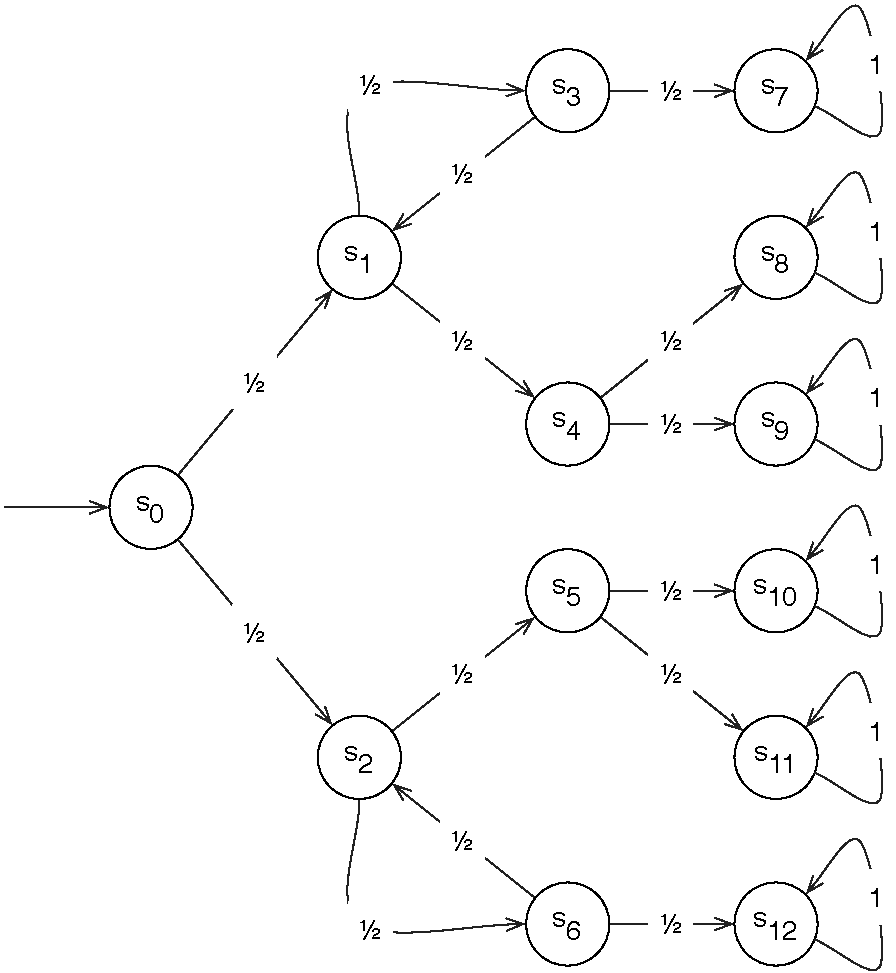
\includegraphics[scale=0.58]{img/example-DTMC.pdf}
\caption[A discrete-time Markov chain example]{The (discrete-time) Markov chain for a six-sided die simulated via a fair coin~\cite{Baier_2008}.}
\label{fig:example_DTMC}
\end{figure}

The DTMC in Figure~\ref{fig:example_DTMC} comprises an initial node $s_0$---such that $\iota_{init}(s_0) = 1$ and $\forall s \neq s_0: \iota_{init}(s) = 0$---and twelve states $S = \{s_1,\ldots,s_{12}\}$. Six inner states $\{s_1,\ldots,s_6\}$ and six terminating states $\{s_7,\ldots,s_{12}\}$ represent the tossing of a coin and possible die outcomes, repsectively. A Markov chain path, which can be rendered as a directed path in the underlying digraph, is a non-empty sequence of states $\pi = s_0\;s_1\;s_2 \cdots \in S^\omega$ such that $\forall i \ge 0: P(s_i, s_{i+1}) > 0$.

For a given DTMC, the transition probability function~$\mathbf{P}$ and the initial distribution $\iota_{init}$ can be represented, respectively, by a transition matrix $\left(\mathbf{P}(s, s')\right)_{s \in S}$ and an initial distribution vector $\left(\iota_{init}(s)\right)_{s \in S}$. The matrix specifies for each state $s \in S$ the probability $\mathbf{P}(s, s')$ of transitioning from~$s$ to~$s'$ in a discrete time-step. The vector specifies for each state $s \in S$ the probability $\iota_{init}(s)$ that the system evolution begins in~$s$. Figure~\ref{fig:transition_matrix_initial_distribution_vector} provides a partial transition matrix and a partial initial distribution vector for the DTMC in Figure~\ref{fig:example_DTMC}.

\setcounter{MaxMatrixCols}{11}

\begin{figure}[ht]
	\begin{equation*}
		\mathbf{P} =
			\begin{array}{c}
				\\
				s_0\\
				s_1\\
				s_2\\
				s_3\\
				s_4\\
				\vdots\\
			\end{array}
			\begin{array}{c}
				\begin{array}{
						c@{\hspace{0.9em}}
						c@{\hspace{0.9em}}
						c@{\hspace{0.9em}}
						c@{\hspace{0.9em}}
						c@{\hspace{0.9em}}
						c@{\hspace{0.9em}}
						c@{\hspace{0.9em}}
						c@{\hspace{0.9em}}
						c@{\hspace{0.9em}}
						c@{\hspace{0.9em}}
						c
					}
					s_0 & s_1 & s_2 & s_3 & s_4 & s_5 & s_6 & s_7 & s_8 & s_9 & \cdots\\
				\end{array}\\
				\left[
					\begin{array}{
							c@{\hspace{1.2em}}
							c@{\hspace{1.2em}}
							c@{\hspace{1.2em}}
							c@{\hspace{1.2em}}
							c@{\hspace{1.2em}}
							c@{\hspace{1.2em}}
							c@{\hspace{1.2em}}
							c@{\hspace{1.2em}}
							c@{\hspace{1.2em}}
							c@{\hspace{1.2em}}
							c
						}
						0 & \frac{1}{2} & \frac{1}{2} & 0 & 0 & 0 & 0 & 0 & 0 & 0 & \cdots\\
						0 & 0 & 0 & \frac{1}{2} & \frac{1}{2} & 0 & 0 & 0 & 0 & 0 & \cdots\\
						0 & 0 & 0 & 0 & 0 & \frac{1}{2} & \frac{1}{2} & 0 & 0 & 0 & \cdots\\
						0 & \frac{1}{2} & 0 & 0 & 0 & 0 & 0 & \frac{1}{2} & 0 & 0 & \cdots\\
						0 & 0 & 0 & 0 & 0 & 0 & 0 & 0 & \frac{1}{2} & \frac{1}{2} & \cdots\\
						\vdots & \vdots & \vdots & \vdots & \vdots & \vdots & \vdots & \vdots & \vdots & \vdots & \ddots\\
					\end{array}
				\right]
			\end{array}
		\iota_{init} =
			\begin{array}{c}
				\\
				s_0\\
				s_1\\
				s_2\\
				s_3\\
				s_4\\
				\vdots\\
			\end{array}
			\begin{array}{c}
				\begin{array}{c}
					\\
				\end{array}\\
				\left[
					\begin{array}{c}
						1\\
						0\\
						0\\
						0\\
						0\\
						\vdots\\
					\end{array}
				\right]
			\end{array}
	\end{equation*}
	\caption[Transition matrix and initial distribution vector examples]{The partial transition matrix and partial initial distribution vector for a six-sided die simulated via a fair coin, as illustrated in Figure~\ref{fig:example_DTMC}.}
	\label{fig:transition_matrix_initial_distribution_vector}
\end{figure}

Probabilistic model checking can be used to verify both quantitative and qualitative DTMC properties. The former constrain probabilities to specific thresholds, while the latter associate desirable and undesirable behavior with probabilities of one and zero, respectively. PCTL is an extension of the branching-time \emph{computation tree logic} (CTL), and a prominent formalism for expressing probabilistic properties. PCTL supports the probabilistic operator $\mathbb{P}_{J}(\varphi)$, where $\varphi$ specifies a constraint over the set of paths that constitute a Markov chain, and $J$ specifies a closed interval between one and zero that bounds the probability of satisfying $\varphi$.

\section{UAV Missions}
\label{sec:UAV_Missions}

UAVs, or \emph{uninhabited aerial systems} (UASs), are aircraft capable of either autonomous or remote controlled flight. Primarily oriented toward (dull, dirty and dangerous) military missions, UAVs are increasingly relied upon to perform agricultural, scientific, industrial and law-enforcement tasks over civilian airspace~\cite{Rango_2010,Jimenez_Berni_2009,Heintz_2007}.

The UAV domain exhibits complexity at different levels of granularity. UAVs incorporate sophisticated payloads, multiple sensors and increasing computational power. These capabilities could, in time, enable UAV swarms to execute complex multi-task missions with reduced human supervision~\cite{Karaman_2008}. Figure~\ref{fig:UAV_autonomy} illustrates various levels of UAV autonomy, ranging from remotely guided drones to fully autonomous swarms, which correspond to levels of automation originally proposed by Sheridan and Verplank~\cite{Nowak_2007}. For any given mission, autonomous UAVs may be required to execute tasks synchronously and in real-time; with local, incomplete and/or noisy knowledge; and in the context of a dynamic environment~\cite{Tosic_2003}. These factors combine to form a complex stochastic state space that motivates the probabilistic verification of UAV mission plans.

\begin{figure}[ht]
\centering
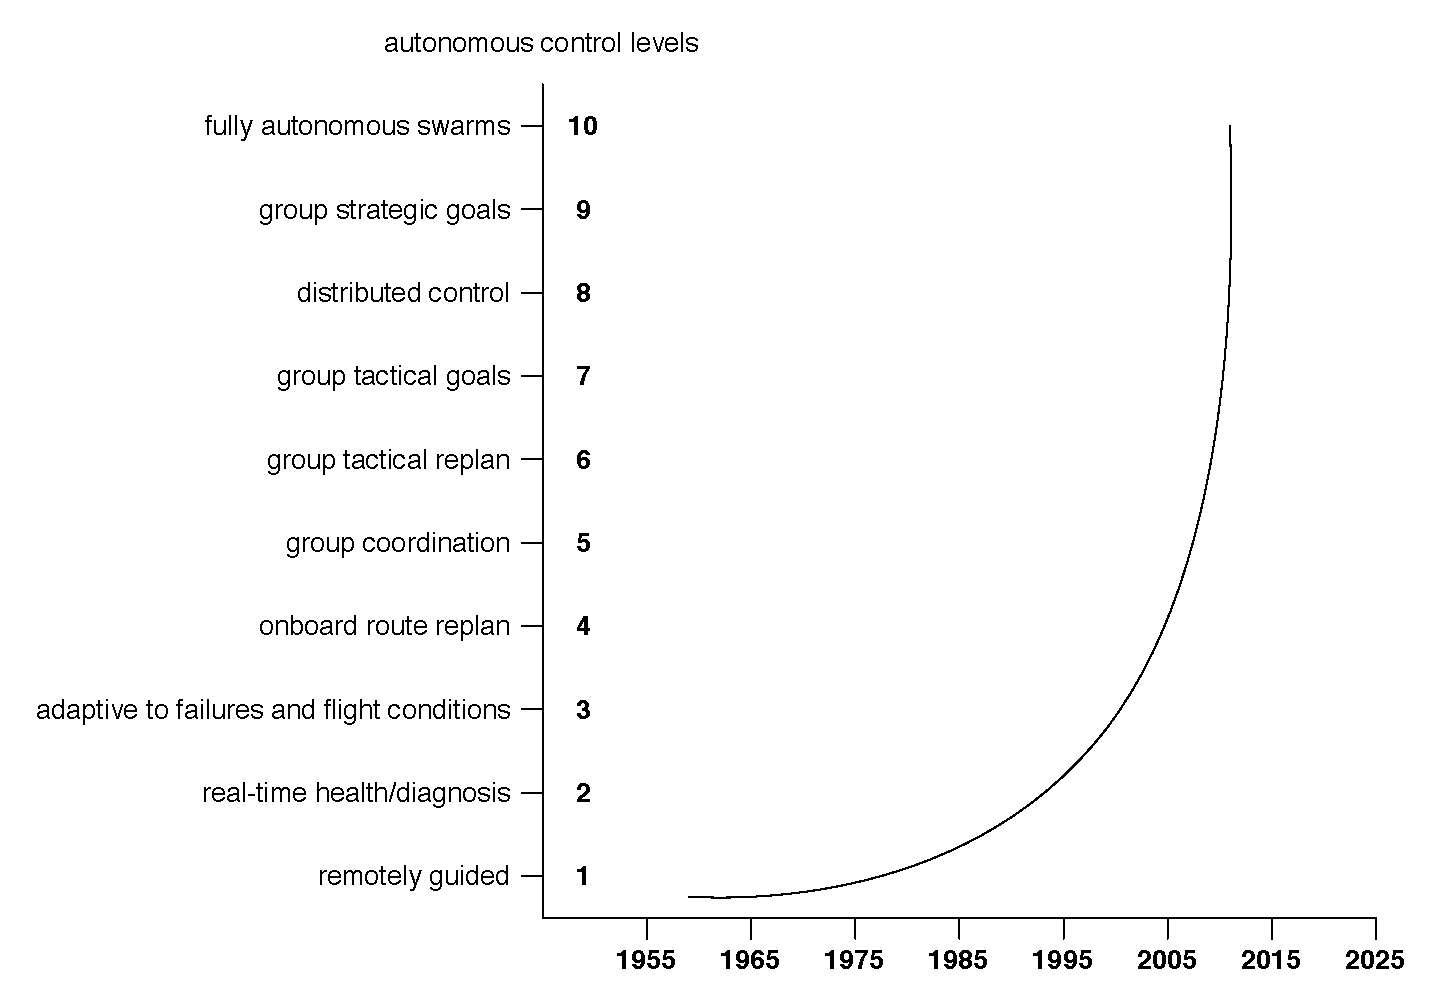
\includegraphics[scale=0.58]{img/UAV-autonomy.pdf}
\caption[UAV autonomy hierarchy]{A hierarchy of UAV autonomy levels~\cite{Youngson_2004,DoD_2005}.}
\label{fig:UAV_autonomy}
\end{figure}

This section provides a concise overview of what is an expansive application domain. Chapter~\ref{chap:Domain_Modeling} explores a subset of that domain in greater detail.

\subsection{UAV Performance Specifications}
\label{sec:UAV_Performance_Specifications}

UAVs can be classified with respect to their performance specifications, and the mission requirements that those specifications are meant to address~\cite{Arjomandi}. UAV performance specifications include the following:

\begin{itemize}

\item \emph{ceiling} (measured in meters), ``an aircraft's maximum pressure height''~\cite{Crocker_2007};

\item \emph{cost};

\item \emph{endurance} (hours), ``the length of time an aircraft can stay in the air without refueling''~\cite{Crocker_2007};

\item \emph{engine type};

\item \emph{payload} (kilograms), ``the load carried by an aircraft''~\cite{Crocker_2007};

\item \emph{power} (kilowatt), ``the propulsive power needed to produce thrust''~\cite{Crocker_2007};

\item \emph{range} (kilometers), ``the maximum distance an aircraft can fly on a given amount of fuel''~\cite{Crocker_2007};

\item \emph{speed} (kilometers per hour);

\item \emph{weight} (kilograms);

\item \emph{wing loading} ($\textrm{kg/m}^2$), ``the weight of an aircraft per unit wing area''~\cite{Crocker_2007};

\item \emph{wing span} (meters), ``a measurement from the tip of one wing to the tip of the other wing''~\cite{Crocker_2007}.

\end{itemize}

Table~\ref{tab:UAV_performance_specifications} lists the performance specifications for various active (at the time of writing) military- and commercial-grade UAVs~\cite{Arjomandi,AscTec,Draganfly,Parrot}. The range of values encompassed by each performance specification can be divided into categories~\cite{Arjomandi}. Table~\ref{tab:UAV_performance_specification_categories} uses these categories to classify a subset of the UAVs listed in Table~\ref{tab:UAV_performance_specifications}.

\begin{sidewaystable}
	\centering
	\arrayrulecolor{Gray}
	\renewcommand*\arraystretch{1.3}
	\begin{tabular}{ l l | c c c c c c c c c }
		\multirow{2}{*}{\emph{UAV}} &
			\multirow{2}{*}{\emph{manufacturer}} &
			\emph{ceiling} &
			\emph{endurance} &
			\emph{payload} &
			\emph{range} &
			\emph{speed} &
			\emph{weight} &
			\emph{wing loading} &
			\emph{wing span}\\
			& & (m) & (hr) & (kg) & (km) & (km/h) & (kg) & ($\textrm{kg/m}^2$) & (m)\\
		\hline
		BQM-147 Dragon & BAI Aerosystems & 3,048 & 3 & 11 & 148 & 160 & 41 & 22 & 2\\
		Crecerelle & SAGEM & 3,353 & 6 & 35 & 59 & 246 & 120 & 9 & 3\\
		Heron (Machatz-1) & Israel Aerospace Industries & 10,000 & 40 & 227 & 3,300 & 207 & 1,087 & 70 & 17\\
		Luna X-2000 & EMT Penzberg & 4,000 & 4 & 10 & 80 & 160 & 40 & 40 & 4\\
		MQ-1 Predator & General Atomics & 7,920 & 20 & 600 & 740 & 217 & 1,020 & 89 & 15\\
		MQ-8 Fire Scout & Northrop Grumman & 6,096 & 6 & 90 & 400 & 231 & 1,159 & 69 & 9\\
		MQ-9 Reaper & General Atomics & 15,200 & 24 & 3,000 & 1,500 & 405 & 4,500 & 83 & 20\\
		RQ-2 Pioneer & AAI Corporation & 4,572 & 5 & 64 & 373 & 175 & 125 & 34 & 5\\
		RQ-4 Global Hawk & Northrop Grumman & 20,000 & 30 & 900 & 22,000 & 636 & 11,600 & 199 & 35\\
		RQ-7 Shadow & AAI Corporation & 4,270 & 5 & 75 & 125 & 204 & 149 & 79 & 4\\
		RQ-11 Raven & AeroVironment & 4,267 & 4 & 17 & 100 & 204 & 84 & 57 & 3\\
		RQ-14 Dragon Eye & AeroVironment & 305 & 1 & 0 & 5 & 65 & 2 & 5 & 1\\
		RQ-15 Neptune & DRS Technologies & 2,440 & 4 & 10 & 75 & 156 & 36 & 74 & 2\\
		\hline
		AR.Drone 1.0 & Parrot & 6--50 & 0.2 & 0 & 0.05--0.335 & 18 & 0.38--0.42 & n/a & n/a\\
		Falcon 8 & AscTec & 2,500 & 0.27--0.3 & 0.5 & 0.15 & 10.8--54 & 0.8 & n/a & n/a\\
		X6 & Draganfly & 2,438 & n/a & 0.5 & n/a & 50 & 1 & n/a & n/a\\
	\end{tabular}
	\caption[UAV performance specifications]{Performance specifications for various military- and commercial-grade UAVs (top and bottom, respectively) including the established MQ-1 Predator and MQ-9 Reaper from General Atomics; and the MQ-8 Fire Scout helicopter from Northrop Grumman.}
	\label{tab:UAV_performance_specifications}
\end{sidewaystable}

\begin{table}[ht]
	\arrayrulecolor{Gray}
	\renewcommand*\arraystretch{1.3}
	\begin{tabularx}{\textwidth}{
			>{\centering\hsize=0.3\hsize}X|
			>{\centering\hsize=0.2\hsize}X|
			>{\centering\hsize=0.2\hsize}X|
			>{\centering\hsize=0.3\hsize}X
		}
		\emph{specification} &
			\emph{category} &
			\emph{range} &
			\emph{UAV}\tabularnewline
		\hline
		\multirow{3}{*}{\emph{ceiling} (m)}
			& low & $<$1000 & RQ-14 Dragon Eye\tabularnewline
			& medium & 1000--10,000 & MQ-1 Predator\tabularnewline
			& high & $>$10,000 & RQ-4 Global Hawk\tabularnewline
		\hline
		\multirow{3}{*}{\emph{endurance} (hr)}
			& low & $<$5 & RQ-14 Dragon Eye\tabularnewline
			& medium & 5--24 & MQ-1 Predator\tabularnewline
			& high & $>$24 & RQ-4 Global Hawk\tabularnewline
		\hline
		\multirow{3}{*}{\emph{range} (km)}
			& low & $<$100 & RQ-14 Dragon Eye\tabularnewline
			& medium & 100--1500 & MQ-1 Predator\tabularnewline
			& high & $>$1500 & RQ-4 Global Hawk\tabularnewline
		\hline
		\multirow{5}{*}{\emph{weight} (kg)}
			& micro & $<$5 & RQ-14 Dragon Eye\tabularnewline
			& light & 5--50 & RQ-15 Neptune\tabularnewline
			& medium & 50--200 & RQ-11 Raven\tabularnewline
			& heavy & 200--2000 & MQ-1 Predator\tabularnewline
			& super heavy & $>$2000 & RQ-4 Global Hawk\tabularnewline
		\hline
		\multirow{3}{*}{\emph{wing loading} ($\textrm{kg/m}^2$)}
			& low & $<$50 & RQ-14 Dragon Eye\tabularnewline
			& medium & 50--100 & MQ-1 Predator\tabularnewline
			& high & $>$100 & RQ-4 Global Hawk\tabularnewline
	\end{tabularx}
	\caption[UAV performance specification categories]{Performance specification categories with their respective ranges, and illustrative UAV classifications.}
	\label{tab:UAV_performance_specification_categories}
\end{table}

UAVs can also be classified with respect to the following mission aspects, which categorize mission requirements.

\begin{itemize}

\item \emph{Aerial delivery and resupply} requires UAVs to supply special forces teams covertly and precisely with small quantities of cargo including batteries, water and leaflets for psychological operations~\cite{DoD_2005}.

\item \emph{Combat} requires highly maneuverable \emph{unmanned combat aerial vehicles} (UCAVs) to engage in both air-to-air and air-to-surface combat~\cite{Arjomandi}.

\item \emph{Intelligence, surveillance, target acquisition and reconnaissance} (ISTAR) requires UAVs to enhance situational awareness by collecting battlefield information.

\item \emph{Multi-purpose} requires UAVs to conduct armed reconnaissance against critical and perishable targets.

\item \emph{Radar and communication relay} requires \emph{airborne communication nodes} (ACNs) to ensure information superiority by extending and enhancing tactical intra-theater communications~\cite{DoD_2005}.

\item \emph{Vertical take-off and landing} (VTOL) requires UAVs to generate sufficient downward thrust to takeoff, hover and land within very limited space.

\end{itemize}

The performance specification categories that classify each UAV address a particular set of mission aspects~\cite{Arjomandi}. For example, the MQ-1 Predator is classified as a medium altitude (1000--10,000 meters), medium endurance (5--24 hours), medium range (100--400 km) and heavy weight (200--2000 kg) UAV\@. These classifications determine the Predator to be highly-desirable for ISTAR and multi-purpose missions, and unsuitable for all remaining mission aspects. Table~\ref{tab:UAV_classifications} classifies the military-grade UAVs listed in Table~\ref{tab:UAV_performance_specifications} with a rating scale of zero to four, where zero indicates the inability of a UAV to perform a specific mission aspect; and values in the range of one to four indicate the degree of compatibility, from lowest to highest, respectively, between performance specifications that parameterize UAVs and the performance specifications required by mission aspects.

\begin{table}[ht]
	\arrayrulecolor{Gray}
	\renewcommand*\arraystretch{1.3}
	\begin{tabularx}{\textwidth}{
			>{\raggedright\hsize=0.29\hsize}X|
			>{\centering\hsize=0.13\hsize}X
			>{\centering\hsize=0.13\hsize}X
			>{\centering\hsize=0.13\hsize}X
			>{\centering\hsize=0.19\hsize}X
			>{\centering\hsize=0.13\hsize}X
		}
		& \emph{delivery} &
			\emph{UCAV} &
			\emph{ISTAR} &
			\emph{multi-purpose} &
			\emph{ACN}\tabularnewline
		\hline
		BQM-147 Dragon & 0 & 0 & 0 & 0 & 0\tabularnewline
		Crecerelle & 0 & 0 & 0 & 0 & 0\tabularnewline
		Heron (Machatz-1) & 0 & 0 & 3 & 0 & 0\tabularnewline
		Luna X-2000 & 0 & 0 & 1 & 0 & 0\tabularnewline
		MQ-1 Predator & 0 & 0 & 3 & 4 & 0\tabularnewline
		MQ-8 Fire Scout & 0 & 0 & 0 & 0 & 2\tabularnewline
		MQ-9 Reaper & 0 & 0 & 0 & 0 & 0\tabularnewline
		RQ-2 Pioneer & 0 & 0 & 1.5 & 0 & 0\tabularnewline
		RQ-4 Global Hawk & 0 & 0 & 4 & 0 & 0\tabularnewline
		RQ-7 Shadow & 0 & 0 & 1.5 & 0 & 0\tabularnewline
		RQ-11 Raven & 0 & 0 & 0 & 0 & 0\tabularnewline
		RQ-14 Dragon Eye & 0 & 0 & 1 & 0 & 0\tabularnewline
		RQ-15 Neptune & 0 & 0 & 1 & 0 & 0\tabularnewline
	\end{tabularx}
	\caption[UAV classifications]{UAV classifications with respect to the degree of compatibility between performance specifications that parameterize UAVs and the performance specifications required by (abbreviated) mission aspects. Compatibility is rated with a scale of zero to four, where zero indicates the inability of a UAV to perform a specific mission aspect.}
	\label{tab:UAV_classifications}
\end{table}

\subsection{UAV Mission Hierarchy}
\label{sec:UAV_Mission_Hierarchy}

We distinguish mission aspect from mission; the former is a conceptualization of related mission requirements, the latter a structured collection of interrelated tasks. Table~\ref{tab:mission_hierarchy} presents a tabular hierarchy of military and commercial UAV missions~\cite{Nehme_2006}. High-level missions, which correspond partially to the mission aspects presented in Section~\ref{sec:UAV_Performance_Specifications}, include the following:

\begin{itemize}

\item \emph{communication}, the relay of voice and data between units, and from units to a higher command;

\item \emph{drones}, the imitation of fighter aircraft or other objects for the purposes of training or (enemy) deception;

\item \emph{extraction}, the removal (including search and rescue) of personnel and cargo from a specified target;

\item \emph{insertion}, the delivery of lethal and non-lethal payloads (for example, emergency supplies) to a specified target;

\item \emph{intelligence}, the accumulation, analysis and dissemination of enemy, terrain and weather information in areas of interest or operation;

\item \emph{reconnaissance}, the exploration or inspection of a specific area for the purpose of information gathering;

\item \emph{surveillance}, the (often clandestine) monitoring of behavior and activities;

\item \emph{transport}, the movement or transfer of personnel and cargo between two locations.

\end{itemize}

\definecolor{E1E1E1}{RGB}{225,225,225}
\definecolor{F1F1F1}{RGB}{241,241,241}

\begin{table}[!ht]
	\arrayrulecolor{Gray}
	\renewcommand*\arraystretch{1.3}
	\begin{tabularx}{\textwidth}{ X | X | X }
		\emph{level 1} & \emph{level 2} & \emph{level 3}\\
		\hline
		\multicolumn{3}{ >{\columncolor{E1E1E1}}l }{drones}\\
		\hline
		& \multicolumn{2}{ >{\columncolor{F1F1F1}}l }{decoy}\\
		\hline
		& \multicolumn{2}{ >{\columncolor{F1F1F1}}l }{target practice}\\
		\hline
		\multicolumn{3}{ >{\columncolor{E1E1E1}}l }{communication}\\
		\hline
		\multicolumn{3}{ >{\columncolor{E1E1E1}}l }{extraction}\\
		\hline
		\multicolumn{3}{ >{\columncolor{E1E1E1}}l }{insertion}\\
		\hline
		& \multicolumn{2}{ >{\columncolor{F1F1F1}}l }{electronic warfare}\\
		\hline
		& & electronic attack\\
		\hline
		& & electronic protection\\
		\hline
		& \multicolumn{2}{ >{\columncolor{F1F1F1}}l }{payload delivery}\\
		\hline
		& & lethal\\
		\hline
		& & non-lethal\\
		\hline
		\multicolumn{3}{ >{\columncolor{E1E1E1}}l }{intelligence/reconnaissance}\\
		\hline
		& \multicolumn{2}{ >{\columncolor{F1F1F1}}l }{BDA}\\
		\hline
		& \multicolumn{2}{ >{\columncolor{F1F1F1}}l }{mapping}\\
		\hline
		& \multicolumn{2}{ >{\columncolor{F1F1F1}}l }{target acquisition}\\
		\hline
		& & dynamic target\\
		\hline
		& & static target\\
		\hline
		& \multicolumn{2}{ >{\columncolor{F1F1F1}}l }{target designation}\\
		\hline
		\multicolumn{3}{ >{\columncolor{E1E1E1}}l }{transport}\\
		\hline
		& \multicolumn{2}{ >{\columncolor{F1F1F1}}l }{cargo}\\
		\hline
		& \multicolumn{2}{ >{\columncolor{F1F1F1}}l }{passengers}\\
		\hline
		\multicolumn{3}{ >{\columncolor{E1E1E1}}l }{surveillance}\\
		\hline
		& \multicolumn{2}{ >{\columncolor{F1F1F1}}l }{geospatial surveillance}\\
		\hline
		& & dynamic target\\
		\hline
		& & static target\\
		\hline
		& \multicolumn{2}{ >{\columncolor{F1F1F1}}l }{listening}\\
		\hline
		& \multicolumn{2}{ >{\columncolor{F1F1F1}}l }{NBC sensing}\\
	\end{tabularx}
	\caption[UAV mission hierarchy]{A tabular UAV mission hierarchy, which includes \emph{battle damage assessment} (BDA) and \emph{nuclear, biological and chemical} (NBC) sensing missions.}
	\label{tab:mission_hierarchy}
\end{table}

Table~\ref{tab:mission_hierarchy} divides the \emph{intelligence, surveillance, and reconnaissance} (ISR) mission space, which is itself a subset of the ISTAR mission aspect, into \emph{intelligence/reconnaissance} and \emph{surveillance} missions. When considered from a different perspective, airborne ISR missions can also be divided into mutually exclusive mission segments including \emph{standoff}, which requires ISR platforms to respect the sovereign airspace of other nations; \emph{over flight}, which authorizes ISR platforms to perform low-risk violations of sovereign airspace, with or without consent from the nation whose airspace is being violated; and \emph{denied}, which exposes ISR platforms to a potentially hostile airspace~\cite{DoD_2005}.

UAV missions in general can be divided into planning, management, and re-planning segments to identify functions that will be assumed by human operators~\cite{Nehme_2006}. For example, drone mission segments comprise the following tasks:

\begin{itemize}

\item \emph{mission planning}, the use of 1) a scheduling mechanism to plan health and status reports, 2) threat area and no-fly zone information to designate the area of deployment, and 3) a decision support mechanism to designate loiter locations;

\item \emph{mission management}, the use of indicators to monitor the health, status and progress of a UAV;

\item \emph{mission re-planning}, the use of path planning to re-designate deployment areas.

\end{itemize}

Given these tasks, drone missions require human operators to supervise path planning, and to monitor the health and status of UAVs. Transport missions extend drone missions by requiring operators to monitor the health and status of passengers. Insertion missions, which are more demanding, require operators to supervise path planning; monitor the health and status of the UAV; monitor the status of weapons; identify targets; allocate and schedule resources; and negotiate with, and notify, other stakeholders. Nehme et al.\ provide a comprehensive discussion on UAV missions, and the function of human operators with respect to those missions~\cite{Nehme_2006}.

We have presented UAV missions from multiple perspectives, which support the analysis of mission scenarios at different levels of granularity (from high-level mission objectives with tactical and political implications to low-level tasks performed by human operators). Section~\ref{sec:DARPA_Mission_Scenario} and Section~\ref{sec:DRDC_Mission_Scenario} introduce two illustrative mission scenarios.

\subsection{DARPA Mission Scenario}
\label{sec:DARPA_Mission_Scenario}

UAVForge was a collaborative initiative by DARPA and the Space and Naval Warfare Systems Center Atlantic (SSC Atlantic)~\cite{DARPA}. The aim of the initiative was to crowd-source the design and development of a remotely operated micro-UAV that could be transported in a rucksack by a single person traveling on foot. Submitted UAVs were evaluated in the context of a mission scenario, which involved the observation of suspicious activities occurring in the vicinity of two nondescript urban buildings. Total mission time did not exceed five and a half hours including three hours for the observation task. UAVs were required to demonstrate the following capabilities:

\begin{itemize}

\item vertical take-off(s) from, and landing(s) to, different stationary locations;

\item safe flight within an altitude window of 5--1000 feet, with up to 15 mile per hour winds and 40--100\textdegree F temperatures;

\item point-to-point navigation within 500 feet of defined flight corridors;

\item operation within an assigned airspace and avoidance of defined no-fly zones;

\item (preferably autonomous) avoidance of static and (potentially) dynamic obstacles---including buildings, water towers, and trees---during approach into an observation area;

\item landing in an area similar to a rooftop structure containing \emph{heating, ventilation, and air conditioning} (HVAC) equipment, communications gear, satellite dishes and poles;

\item identification of a vantage point---up to 2.0 miles beyond line-of-sight from the starting location---from which to conduct the observation task

\item observation by landing on, adhering to, hanging over, and/or hovering above or below physical structures;

\item real-time transmission of images or video depicting static and mobile items of interest located up to 100 feet from the observing UAV;

\item data link frequency management and data transmission in compliance with rules and authorized frequencies stipulated, respectively, by the Academy of Model Aeronautics (AMA) and the U.S. Federal Communications Commission (FCC).

\end{itemize}

Figure~\ref{fig:UAVForge_competition_course} illustrates the UAVForge mission scenario, which underpins, and thereby lends credibility to, the~58 UAV mission plans developed for this project. These plans in turn support the development and evaluation of our method and prototype.

\begin{sidewaysfigure}
\centering
\includegraphics[scale=1]{img/UAVForge-competition-course.png}
\caption[DARPA's UAVForge mission scenario]{An illustration of DARPA's UAVForge mission scenario~\cite{DARPA}.}
\label{fig:UAVForge_competition_course}
\end{sidewaysfigure}

\subsection{DRDC Mission Scenario}
\label{sec:DRDC_Mission_Scenario}

The DRDC produces mission scenarios to further knowledge on the intersection of UAV/UCAV devices and \emph{intelligent adaptive interfaces} (IAIs), which are technologies for enhancing performance in complex socio-technical environments such as multi-UAV operations~\cite{Hou_2006,Hou_2011}. Mission scenarios employ a suite of UAV platforms---including \emph{medium altitude long endurance} (MALE) UAVs (for example, the MQ-1 Predator\footnote{In contrast to Youngson et al., Arjomandi classifies the MQ-1 Predator as a medium endurance UAV (see Table~\ref{tab:UAV_performance_specification_categories}).}), VTOL Tactical UAVs (VTUAVs), and mini UAVs---to evaluate the impact of IAI constructs on operations within the UAV domain in Canada~\cite{Youngson_2004}. We will focus on a mission scenario involving a \emph{fishery patrol} (FISHPAT) and a \emph{counter-drug operation} (CD OP), which are representative of domestic ISR missions undertaken by Canadian Forces in peacetime (additional domestic operations include disaster recovery, homeland security, long-duration law enforcement surveillance, and search and rescue).

The CD OP is coordinated from the Maritime Forces Atlantic (MARLANT) Headquarters at Canadian Forces Base (CFB) Halifax with support from HMCS Winnipeg. A \emph{ship of interest} (SOI) is initially tracked by US Customs aircraft and a US Coast Guard vessel. In conjunction with this activity, HMCS Montreal, which carries four VTUAVs, is conducting a FISHPAT approximately 180 nautical miles south of Burin in Newfoundland; and HMCS Kingston, which carries two mini UAVs, is conducting a coastal patrol 150 nautical miles southwest of Burin. Mission correctness is complicated by several factors. Tasked assets operate remotely and at great distances from their home bases. Extended transit times and accurate, timely intelligence reports are therefore critical to mission planning, and asset positioning and availability. In addition, the \emph{area of operation} (AOO) experiences weather conditions---including frequent and extensive fog, low cloud cover and precipitation---that limit the utility of \emph{electro-optical} (EO) and \emph{infrared} (IR) sensors.

A timeline of major mission events is divided into seven segments, which are deemed conducive to IAI experimentation. These segments identify periods of excessive operator workload resulting from ``the simultaneous receipt of sensor data \ldots\ [transmitted by] multiple UAVs; dynamic re-tasking of UAVs; transfer of UAV control between agencies; and concurrent control of multiple UAVs.''~\cite{Youngson_2004} Mission segments include the following (all times are Eastern Standard):

{
\parindent=0em
\parskip=\medskipamount

\newcommand{\myindent}[1]{\hangindent=2em\textbf{#1}}

\myindent{0210--0232 hrs}: HMCS Montreal and Viper~01 (a MALE UAV) are re-tasked from a FISHPAT and a training exercise, respectively, to the CD OP\@. Viper~01 is vectored into position by a \emph{mission control element} (MCE) located at CFB Greenwood. Alpha 51, a manned patrol aircraft, is also re-tasked from a training exercise in order to track the SOI\@.

\myindent{0325--0702 hrs}: HMCS Montreal maintains simultaneous control of two VTUAVs (Bingo~61 and Bingo~62) and receives \emph{synthetic aperture radar} (SAR) imagery from Viper~01.

\myindent{0750--0812 hrs}: Ship board and airborne MCEs---for example, HMCS Kingston and Alpha~52, respectively---execute multiple UAV payload (i.e., EO, IR, and SAR) control transfers.

\myindent{1110--1140 hrs}: Alpha~52 controls, dynamically re-tasks and monitors sensor data from two UAVs (Mike~91 and Mike~92) while receiving SAR imagery from Viper~01. This involves Alpha~52 launching Mike~91, and assuming control of Mike~92 from HMCS Kingston.

\myindent{1200--1432 hrs}: HMCS Montreal controls and monitors sensor data from three UAVs (Bingo~63, Bingo~64 and Mike~92) while receiving SAR imagery from Viper~01. This involves HMCS Montreal launching Bingo~64 to replace Bingo~63, and assuming control of Mike~92 from Alpha~52.

\myindent{1440--1525 hrs}: Alpha~52, HMCS Kingston and HMCS Montreal transfer control of UAVs in conjunction with the surveillance of multiple targets.

\myindent{1620--1700 hrs}: UAV sensor operations and frequency of reporting accelerate in response to an increased operational tempo.

}

As with UAVForge, the DRDC scenario underpins mission plans that in turn support the development and evaluation of our method and prototype.

\section{Summary}
\label{sec:Background_Summary}

This chapter presents background material on the technologies that constitute cascading verification. We also provide a broad, concise overview of the UAV domain to contextualize, and convey the inherent complexity of, UAV missions. Some of the information in this overview is never exploited by our work; for example, our prototype implementation of cascading verification does not incorporate the performance specifications and mission hierarchy presented in Section~\ref{sec:UAV_Performance_Specifications} and Section~\ref{sec:UAV_Mission_Hierarchy}, respectively. But this information is nevertheless pertinent because it has informed our research and development efforts. The scope of our prototype with respect to its application domain will be elaborated in subsequent chapters.
